\documentclass{article}\usepackage[]{graphicx}\usepackage[table]{xcolor}
% maxwidth is the original width if it is less than linewidth
% otherwise use linewidth (to make sure the graphics do not exceed the margin)
\makeatletter
\def\maxwidth{ %
  \ifdim\Gin@nat@width>\linewidth
    \linewidth
  \else
    \Gin@nat@width
  \fi
}
\makeatother

\definecolor{fgcolor}{rgb}{0.345, 0.345, 0.345}
\newcommand{\hlnum}[1]{\textcolor[rgb]{0.686,0.059,0.569}{#1}}%
\newcommand{\hlsng}[1]{\textcolor[rgb]{0.192,0.494,0.8}{#1}}%
\newcommand{\hlcom}[1]{\textcolor[rgb]{0.678,0.584,0.686}{\textit{#1}}}%
\newcommand{\hlopt}[1]{\textcolor[rgb]{0,0,0}{#1}}%
\newcommand{\hldef}[1]{\textcolor[rgb]{0.345,0.345,0.345}{#1}}%
\newcommand{\hlkwa}[1]{\textcolor[rgb]{0.161,0.373,0.58}{\textbf{#1}}}%
\newcommand{\hlkwb}[1]{\textcolor[rgb]{0.69,0.353,0.396}{#1}}%
\newcommand{\hlkwc}[1]{\textcolor[rgb]{0.333,0.667,0.333}{#1}}%
\newcommand{\hlkwd}[1]{\textcolor[rgb]{0.737,0.353,0.396}{\textbf{#1}}}%
\let\hlipl\hlkwb

\usepackage{framed}
\makeatletter
\newenvironment{kframe}{%
 \def\at@end@of@kframe{}%
 \ifinner\ifhmode%
  \def\at@end@of@kframe{\end{minipage}}%
  \begin{minipage}{\columnwidth}%
 \fi\fi%
 \def\FrameCommand##1{\hskip\@totalleftmargin \hskip-\fboxsep
 \colorbox{shadecolor}{##1}\hskip-\fboxsep
     % There is no \\@totalrightmargin, so:
     \hskip-\linewidth \hskip-\@totalleftmargin \hskip\columnwidth}%
 \MakeFramed {\advance\hsize-\width
   \@totalleftmargin\z@ \linewidth\hsize
   \@setminipage}}%
 {\par\unskip\endMakeFramed%
 \at@end@of@kframe}
\makeatother

\definecolor{shadecolor}{rgb}{.97, .97, .97}
\definecolor{messagecolor}{rgb}{0, 0, 0}
\definecolor{warningcolor}{rgb}{1, 0, 1}
\definecolor{errorcolor}{rgb}{1, 0, 0}
\newenvironment{knitrout}{}{} % an empty environment to be redefined in TeX

\usepackage{alltt}

\usepackage[utf8]{inputenc}
\usepackage{float}
\usepackage{graphicx}
\usepackage{booktabs}
\usepackage[table]{xcolor}
\IfFileExists{upquote.sty}{\usepackage{upquote}}{}
\begin{document}
modificacion desde github desktop\\
Se realizara el analisis de las encuestas de todas la encuestas realizadas en el trabajo de campo.\\
\begin{table}[H]
  \centering
  \caption{Edad de los encuestados}

\begin{tabular}{lcl}
\toprule
\cellcolor[HTML]{87A96B}{\textcolor{black}{\textbf{Rango}}} & \cellcolor[HTML]{87A96B}{\textcolor{black}{\textbf{Conteo}}} & \cellcolor[HTML]{87A96B}{\textcolor{black}{\textbf{Porcentaje}}}\\
\midrule
(23.9,33.3] & 28 & 6.35\\
(33.3,42.6] & 54 & 12.24\\
(42.6,51.9] & 87 & 19.73\\
(51.9,61.1] & 127 & 28.80\\
(61.1,70.4] & 97 & 22.00\\
\addlinespace
(70.4,79.7] & 35 & 7.94\\
(79.7,89.1] & 13 & 2.95\\
\bottomrule
\end{tabular}

  \caption*{Fuente trabajo de campo}
\end{table}
Aca ira la interpretacion de la tabla
\begin{figure}[H]
  \centering
  \caption{Porcentaje de edad de los encuestados}
\begin{knitrout}
\definecolor{shadecolor}{rgb}{0.969, 0.969, 0.969}\color{fgcolor}
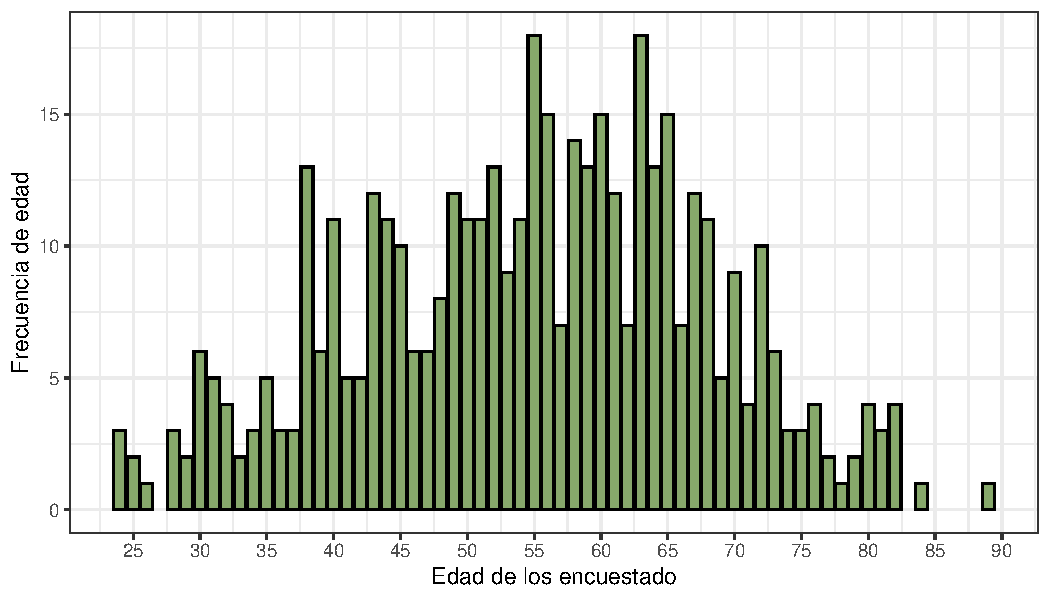
\includegraphics[width=\maxwidth]{figure/fig_uno-1} 
\end{knitrout}
  \caption*{Fuente: trabajo de campo}
\end{figure}
mas interpretacion de la grafica\\
aca se inserta la imagen


\begin{figure}[H]
  \centering
  \caption{Aplicando encuestas}
  \includegraphics[width=7cm, height=7cm]{H:/Gore Cusco/Geragri/programa/analisis datos/fotos/1.jpg}
  \caption*{Fuente: trabajo de campo}
\end{figure}

Se analizara el genero de los encuestados
\begin{table}[H]
  \centering
  \caption{Genero de los encuestados}

\begin{tabular}{lcl}
\toprule
\cellcolor[HTML]{87A96B}{\textcolor{black}{\textbf{GENERO}}} & \cellcolor[HTML]{87A96B}{\textcolor{black}{\textbf{Conteo}}} & \cellcolor[HTML]{87A96B}{\textcolor{black}{\textbf{Porcentaje}}}\\
\midrule
MUJER & 213 & 47.97\\
VARON & 231 & 52.03\\
\bottomrule
\end{tabular}

  \caption*{Fuente: Trabajo de campo}
\end{table}  

\begin{figure}[H]
  \centering
  \caption{Frecuencia del genero de los encuestados}
\begin{knitrout}
\definecolor{shadecolor}{rgb}{0.969, 0.969, 0.969}\color{fgcolor}
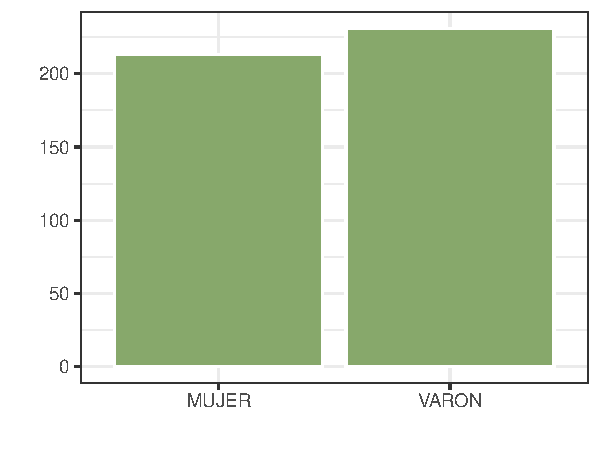
\includegraphics[width=\maxwidth]{figure/fig_dos-1} 
\end{knitrout}
  \caption*{Fuente: Trabajo de campo}
\end{figure}

\begin{table}[H]
  \centering
  \caption{Grado de instruccion}
\begin{kframe}


{\ttfamily\noindent\bfseries\color{errorcolor}{\#\# Error in eval(expr, envir, enclos): objeto 'fil' no encontrado}}\end{kframe}
\begin{tabular}{lcl}
\toprule
\cellcolor[HTML]{87A96B}{\textcolor{black}{\textbf{GENERO}}} & \cellcolor[HTML]{87A96B}{\textcolor{black}{\textbf{Conteo}}} & \cellcolor[HTML]{87A96B}{\textcolor{black}{\textbf{Porcentaje}}}\\
\midrule
MUJER & 213 & 47.97\\
VARON & 231 & 52.03\\
\bottomrule
\end{tabular}

  \caption*{Fuente: Trabajo de campo}
\end{table}

\begin{figure}[H]
  \centering
  \caption{Distribucion del grado de instruccion}
\begin{knitrout}
\definecolor{shadecolor}{rgb}{0.969, 0.969, 0.969}\color{fgcolor}
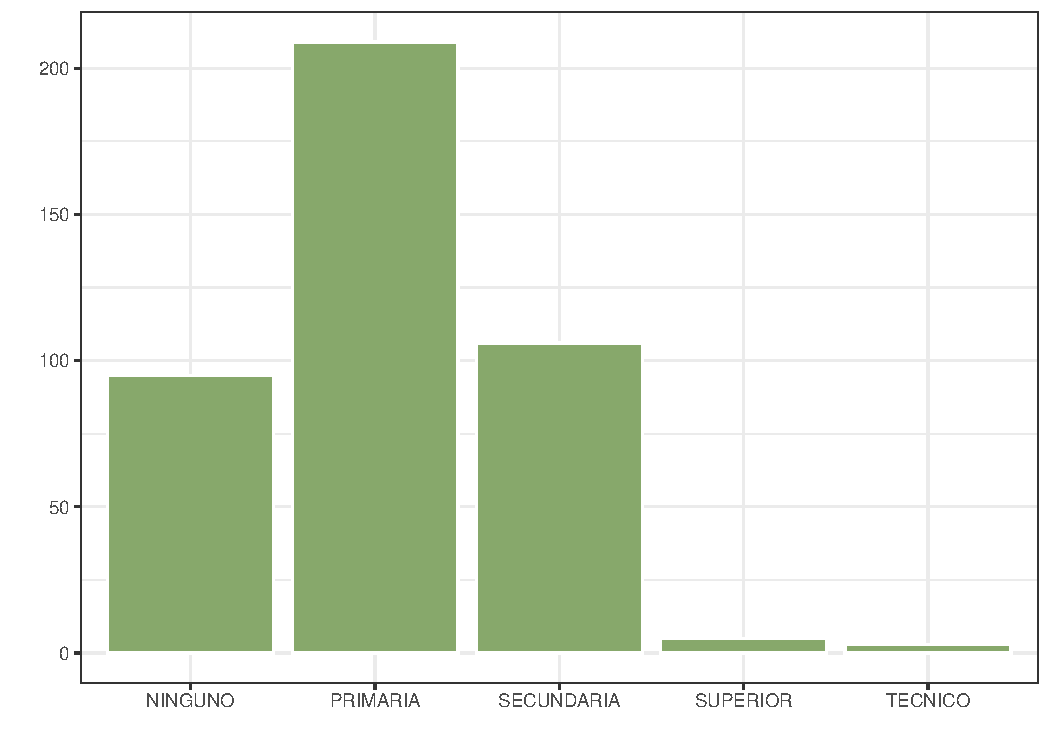
\includegraphics[width=\maxwidth]{figure/fig_tres-1} 
\end{knitrout}
  \caption*{Fuente: Trabajo de campo}
\end{figure}

\begin{figure}[H]
  \centering
  \caption{Aplicando encuestas}
  \includegraphics[width=7cm, height=7cm]{H:/Gore Cusco/Geragri/programa/analisis datos/fotos/2.jpg}
  \caption*{Fuente: trabajo de campo}
\end{figure}


\begin{table}[H]
  \centering
  \caption{Tipo de ingreso familiar}

\begin{tabular}{lcl}
\toprule
\cellcolor[HTML]{87A96B}{\textcolor{black}{\textbf{Ingreso}}} & \cellcolor[HTML]{87A96B}{\textcolor{black}{\textbf{Conteo}}} & \cellcolor[HTML]{87A96B}{\textcolor{black}{\textbf{Porcentaje}}}\\
\midrule
ANUAL & 240 & 61.22\\
MENSUAL & 126 & 32.14\\
QUINCENAL & 20 & 5.10\\
SEMANAL & 6 & 1.53\\
\bottomrule
\end{tabular}

  \caption*{Fuente: Trabajo de campo}
\end{table}


\begin{figure}[H]
  \centering
  \caption{Distribucion del tipo de ingreso familiar}
\begin{knitrout}
\definecolor{shadecolor}{rgb}{0.969, 0.969, 0.969}\color{fgcolor}
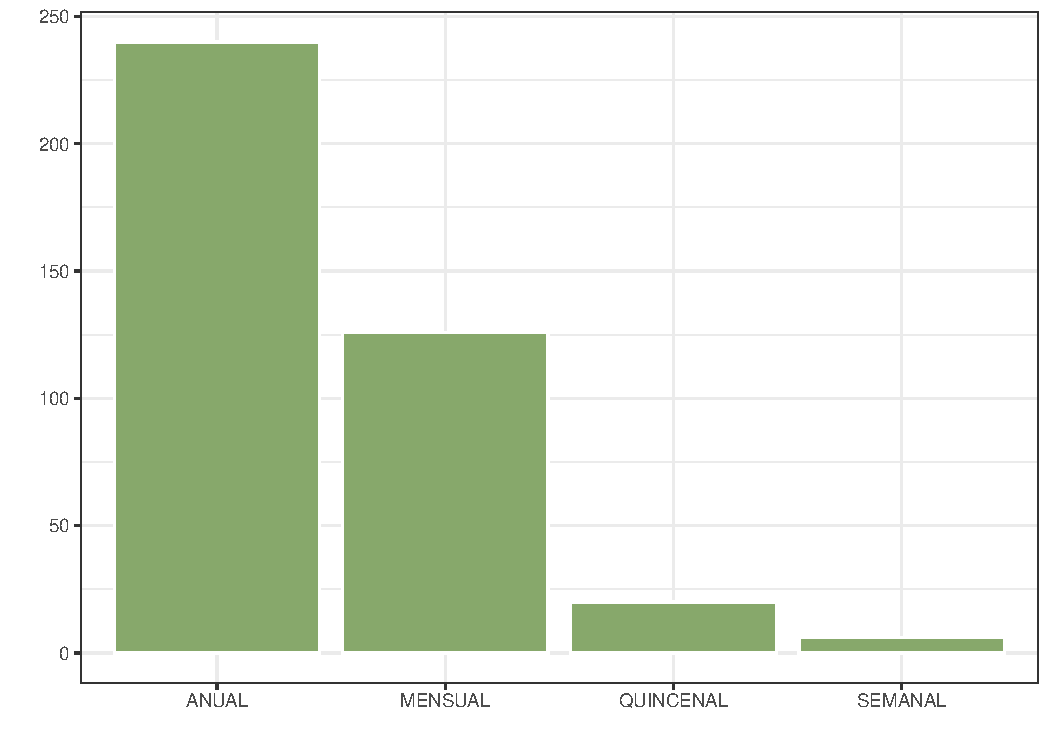
\includegraphics[width=\maxwidth]{figure/fig_cinco-1} 
\end{knitrout}
  \caption*{Fuente: Trabajo de campo}
\end{figure}

\begin{figure}[H]
  \centering
  \caption{Aplicacion de encuestas}
  \includegraphics[width=7cm, height=7cm]{H:/Gore Cusco/Geragri/programa/analisis datos/fotos/3.jpg}
  \caption*{Fuente: trabajo de campo}
\end{figure}

\begin{table}[H]
  \centering
  \caption{Ingreso familiar}

\begin{tabular}{lcl}
\toprule
\cellcolor[HTML]{87A96B}{\textcolor{black}{\textbf{Ingreso\_familiar}}} & \cellcolor[HTML]{87A96B}{\textcolor{black}{\textbf{Conteo}}} & \cellcolor[HTML]{87A96B}{\textcolor{black}{\textbf{Porcentaje}}}\\
\midrule
Mayor a S/1500 & 29 & 7.51\\
S/100 a S/500 & 269 & 69.69\\
S/501 a S/950 & 51 & 13.21\\
S/951 a S/1500 & 37 & 9.59\\
\bottomrule
\end{tabular}

  \caption*{Fuente: Trabajo de campo}
\end{table}


\begin{figure}[H]
  \centering
  \caption{Distribucion del tipo de ingreso familiar}
\begin{knitrout}
\definecolor{shadecolor}{rgb}{0.969, 0.969, 0.969}\color{fgcolor}
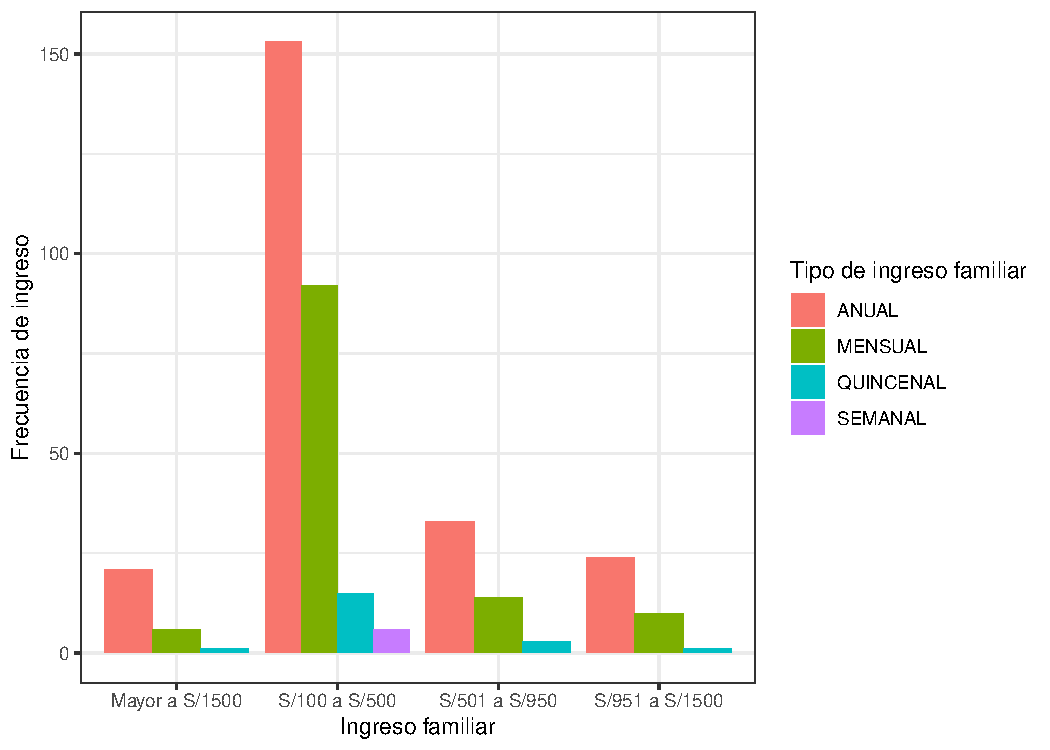
\includegraphics[width=\maxwidth]{figure/fig_seis-1} 
\end{knitrout}
  \caption*{Fuente: Trabajo de campo}
\end{figure}

\begin{figure}[H]
  \centering
  \caption{Sensibililzacion a los beneficiarios}
  \includegraphics[width=7cm, height=7cm]{H:/Gore Cusco/Geragri/programa/analisis datos/fotos/4.jpg}
  \caption*{Fuente: trabajo de campo}
\end{figure}


\begin{table}[H]
  \centering
  \caption{Numero de integrantes que conforman su familia}

\begin{tabular}{lcl}
\toprule
\cellcolor[HTML]{87A96B}{\textcolor{black}{\textbf{Integrantes}}} & \cellcolor[HTML]{87A96B}{\textcolor{black}{\textbf{Conteo}}} & \cellcolor[HTML]{87A96B}{\textcolor{black}{\textbf{Porcentaje}}}\\
\midrule
 & 7 & 1.55\\
3 A 5 PERSONAS & 228 & 50.55\\
MAS DE 6 PERSONAS & 41 & 9.09\\
MENOS DE 2 PERSONAS & 175 & 38.80\\
\bottomrule
\end{tabular}

  \caption*{Fuente: Trabajo de campo}
\end{table}

\begin{figure}[H]
  \centering
  \caption{Distribucion del tipo de ingreso familiar}
\begin{knitrout}
\definecolor{shadecolor}{rgb}{0.969, 0.969, 0.969}\color{fgcolor}
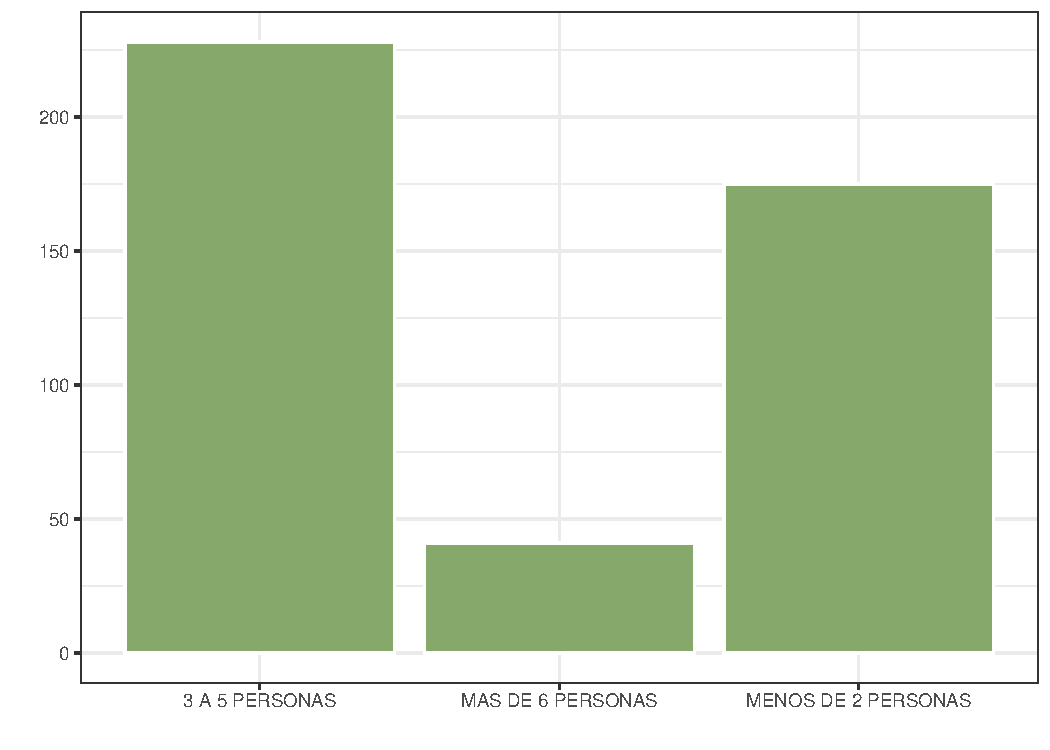
\includegraphics[width=\maxwidth]{figure/fig_siete-1} 
\end{knitrout}
  \caption*{Fuente: Trabajo de campo}
\end{figure}

\begin{figure}[H]
  \centering
  \caption{Sensibililzacion a los beneficiarios}
  \includegraphics[width=7cm, height=7cm]{H:/Gore Cusco/Geragri/programa/analisis datos/fotos/5.jpg}
  \caption*{Fuente: trabajo de campo}
\end{figure}


\begin{table}[H]
  \centering
  \caption{Actividad economica a la que se dedica}

\begin{tabular}{lcl}
\toprule
\cellcolor[HTML]{87A96B}{\textcolor{black}{\textbf{Actividad}}} & \cellcolor[HTML]{87A96B}{\textcolor{black}{\textbf{Conteo}}} & \cellcolor[HTML]{87A96B}{\textcolor{black}{\textbf{Porcentaje}}}\\
\midrule
AGRICULTOR & 146 & 32.74\\
AGROPECUARIO & 156 & 34.98\\
AMA DE CASA & 126 & 28.25\\
COMERCIANTE & 6 & 1.35\\
PECUARIO & 8 & 1.79\\
\addlinespace
TRABAJADOR PUBLICO & 4 & 0.90\\
\bottomrule
\end{tabular}

  \caption*{Fuente: Trabajo de campo}
\end{table}

\begin{figure}[H]
  \centering
  \caption{Actividad economica a la que se dedica}
\begin{knitrout}
\definecolor{shadecolor}{rgb}{0.969, 0.969, 0.969}\color{fgcolor}
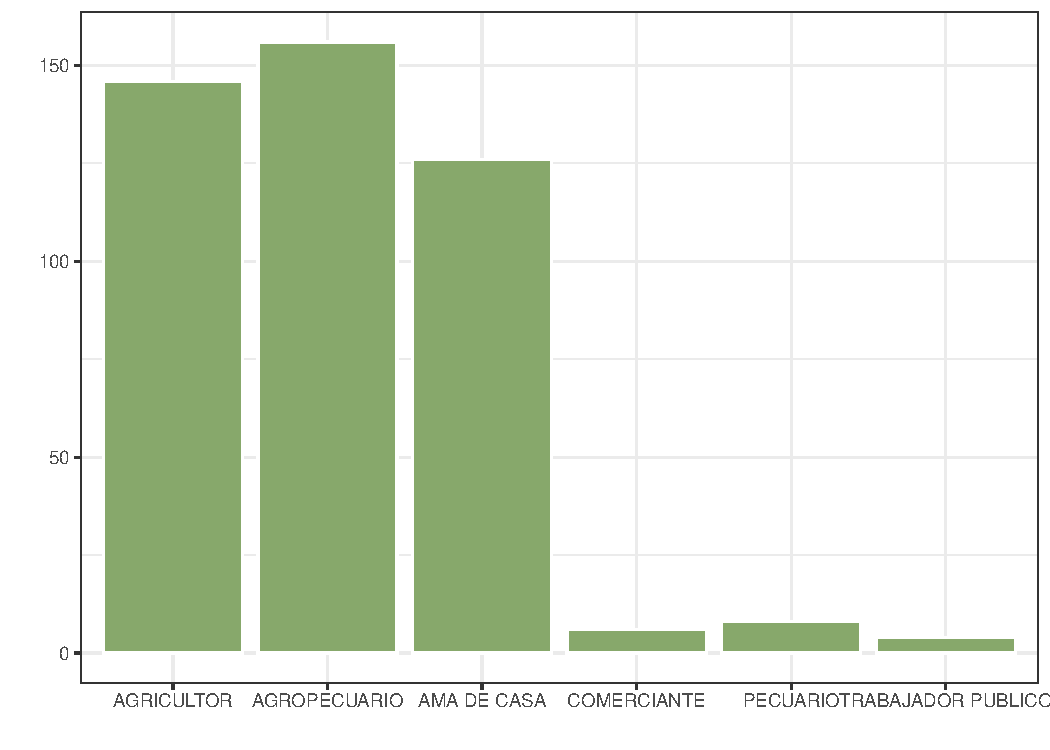
\includegraphics[width=\maxwidth]{figure/fig_ocho-1} 
\end{knitrout}
  \caption*{Fuente: Trabajo de campo}
\end{figure}

\begin{figure}[H]
  \centering
  \caption{Aplicacion de encuestas en el area de influencia}
  \includegraphics[width=7cm, height=7cm]{H:/Gore Cusco/Geragri/programa/analisis datos/fotos/6.jpg}
  \caption*{Fuente: trabajo de campo}
\end{figure}


\begin{table}[H]
  \centering
  \caption{Cuenta con el servicio de agua potable}

\begin{tabular}{lcl}
\toprule
\cellcolor[HTML]{87A96B}{\textcolor{black}{\textbf{Agua}}} & \cellcolor[HTML]{87A96B}{\textcolor{black}{\textbf{Conteo}}} & \cellcolor[HTML]{87A96B}{\textcolor{black}{\textbf{Porcentaje}}}\\
\midrule
NO & 3 & 0.67\\
SI & 445 & 99.33\\
\bottomrule
\end{tabular}

  \caption*{Fuente: Trabajo de campo}
\end{table}

\begin{figure}[H]
  \centering
  \caption{Cuenta con el servicio de agua potable}
\begin{knitrout}
\definecolor{shadecolor}{rgb}{0.969, 0.969, 0.969}\color{fgcolor}
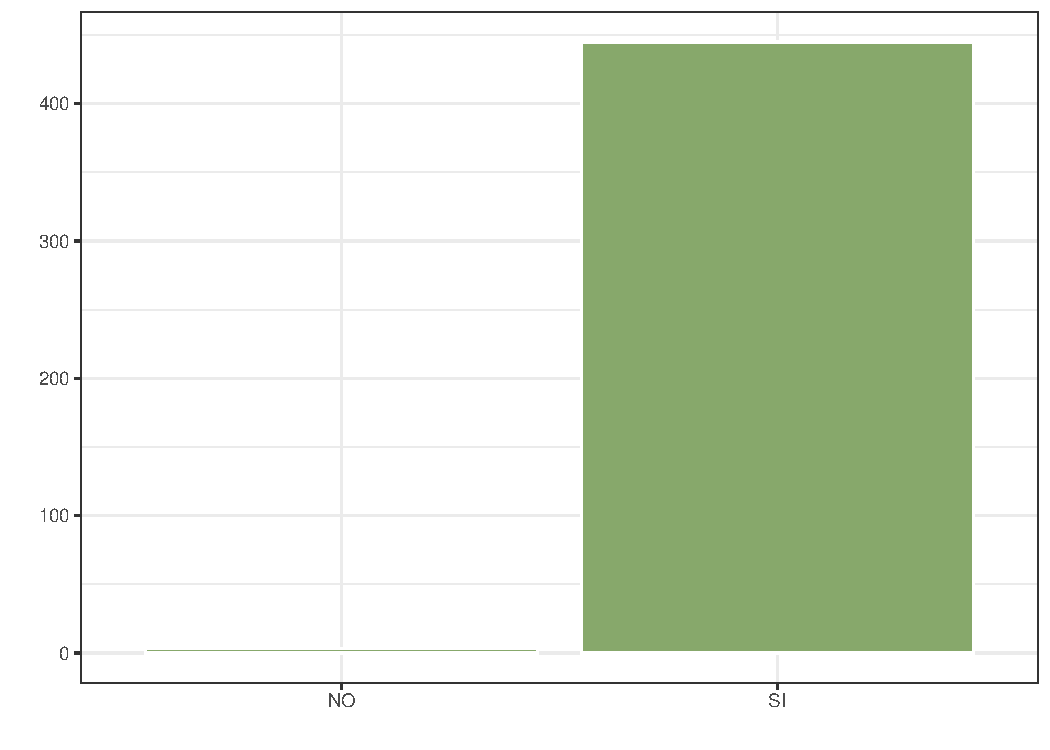
\includegraphics[width=\maxwidth]{figure/fig_nueve-1} 
\end{knitrout}
  \caption*{Fuente: Trabajo de campo}
\end{figure}

\begin{figure}[H]
  \centering
  \caption{Aplicacion de encuestas en el area de influencia}
  \includegraphics[width=7cm, height=7cm]{H:/Gore Cusco/Geragri/programa/analisis datos/fotos/7.jpg}
  \caption*{Fuente: trabajo de campo}
\end{figure}


\begin{table}[H]
  \centering
  \caption{Cuenta con el servicio de agua potable}

\begin{tabular}{lcl}
\toprule
\cellcolor[HTML]{87A96B}{\textcolor{black}{\textbf{Agua\_que\_consume}}} & \cellcolor[HTML]{87A96B}{\textcolor{black}{\textbf{Conteo}}} & \cellcolor[HTML]{87A96B}{\textcolor{black}{\textbf{Porcentaje}}}\\
\midrule
CLORADA & 327 & 75.00\\
POTABLE & 91 & 20.87\\
SIN TRATAR & 18 & 4.13\\
\bottomrule
\end{tabular}

  \caption*{Fuente: Trabajo de campo}
\end{table}

\begin{figure}[H]
  \centering
  \caption{Cuenta con el servicio de agua potable}
\begin{knitrout}
\definecolor{shadecolor}{rgb}{0.969, 0.969, 0.969}\color{fgcolor}
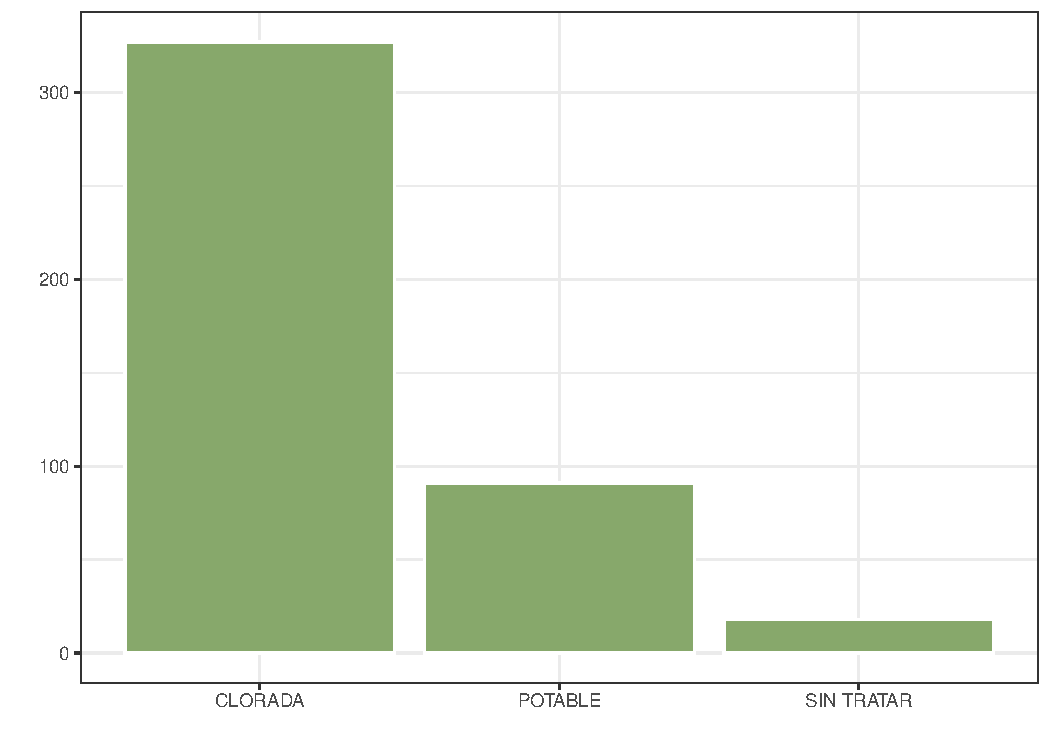
\includegraphics[width=\maxwidth]{figure/fig_diez-1} 
\end{knitrout}
  \caption*{Fuente: Trabajo de campo}
\end{figure}

\begin{figure}[H]
  \centering
  \caption{Aplicacion de encuestas en el area de influencia}
  \includegraphics[width=7cm, height=7cm]{H:/Gore Cusco/Geragri/programa/analisis datos/fotos/8.jpg}
  \caption*{Fuente: trabajo de campo}
\end{figure}




\begin{table}[H]
  \centering
  \caption{Abastecimiento de agua}

\begin{tabular}{lcl}
\toprule
\cellcolor[HTML]{87A96B}{\textcolor{black}{\textbf{Abastecimiento\_agua}}} & \cellcolor[HTML]{87A96B}{\textcolor{black}{\textbf{Conteo}}} & \cellcolor[HTML]{87A96B}{\textcolor{black}{\textbf{Porcentaje}}}\\
\midrule
MANTIAL & 323 & 72.91\\
PILON DE USO PUBLICO & 13 & 2.93\\
RED PUBLICA & 94 & 21.22\\
RIO O RIACHUELO & 13 & 2.93\\
\bottomrule
\end{tabular}

  \caption*{Fuente: Trabajo de campo}
\end{table}

\begin{figure}[H]
  \centering
  \caption{Fuente de abastecimiento de agua}
\begin{knitrout}
\definecolor{shadecolor}{rgb}{0.969, 0.969, 0.969}\color{fgcolor}
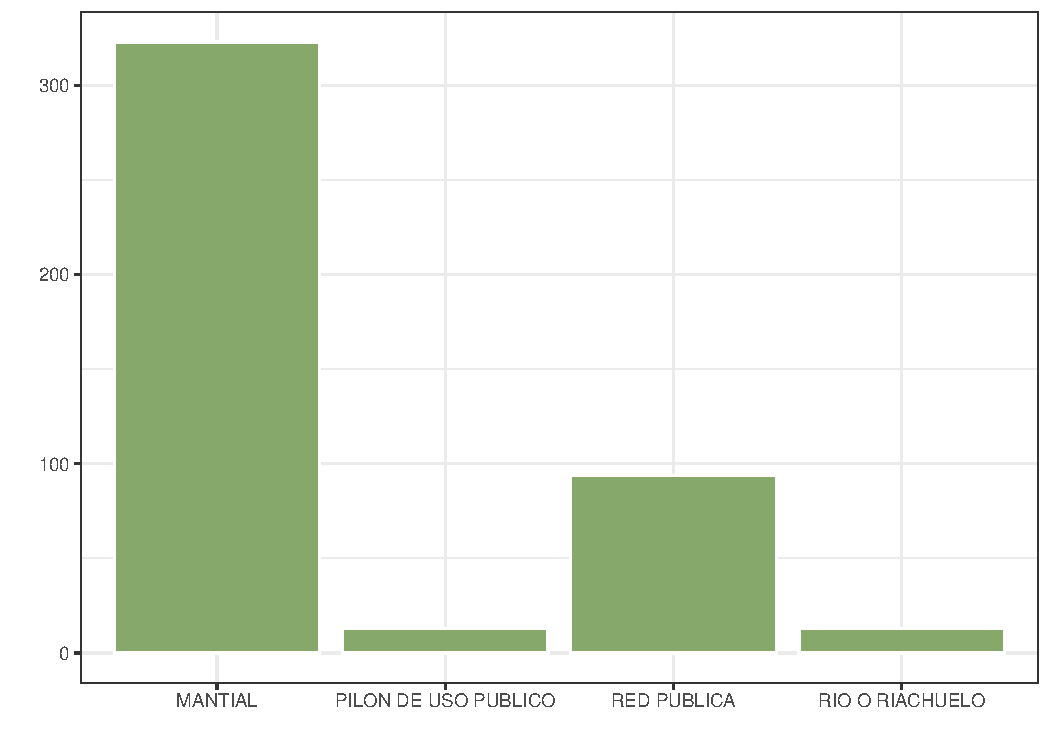
\includegraphics[width=\maxwidth]{figure/fig_once-1} 
\end{knitrout}
  \caption*{Fuente: Trabajo de campo}
\end{figure}

\begin{figure}[H]
  \centering
  \caption{Sensibilizacion a los productores}
  \includegraphics[width=7cm, height=7cm]{H:/Gore Cusco/Geragri/programa/analisis datos/fotos/9.jpg}
  \caption*{Fuente: trabajo de campo}
\end{figure}


\begin{table}[H]
  \centering
  \caption{Energia electrica}

\begin{tabular}{lcl}
\toprule
\cellcolor[HTML]{87A96B}{\textcolor{black}{\textbf{Electricidad}}} & \cellcolor[HTML]{87A96B}{\textcolor{black}{\textbf{Conteo}}} & \cellcolor[HTML]{87A96B}{\textcolor{black}{\textbf{Porcentaje}}}\\
\midrule
NO & 26 & 5.83\\
SI & 420 & 94.17\\
\bottomrule
\end{tabular}

  \caption*{Fuente: Trabajo de campo}
\end{table}

\begin{figure}[H]
  \centering
  \caption{Energia electrica}
\begin{knitrout}
\definecolor{shadecolor}{rgb}{0.969, 0.969, 0.969}\color{fgcolor}
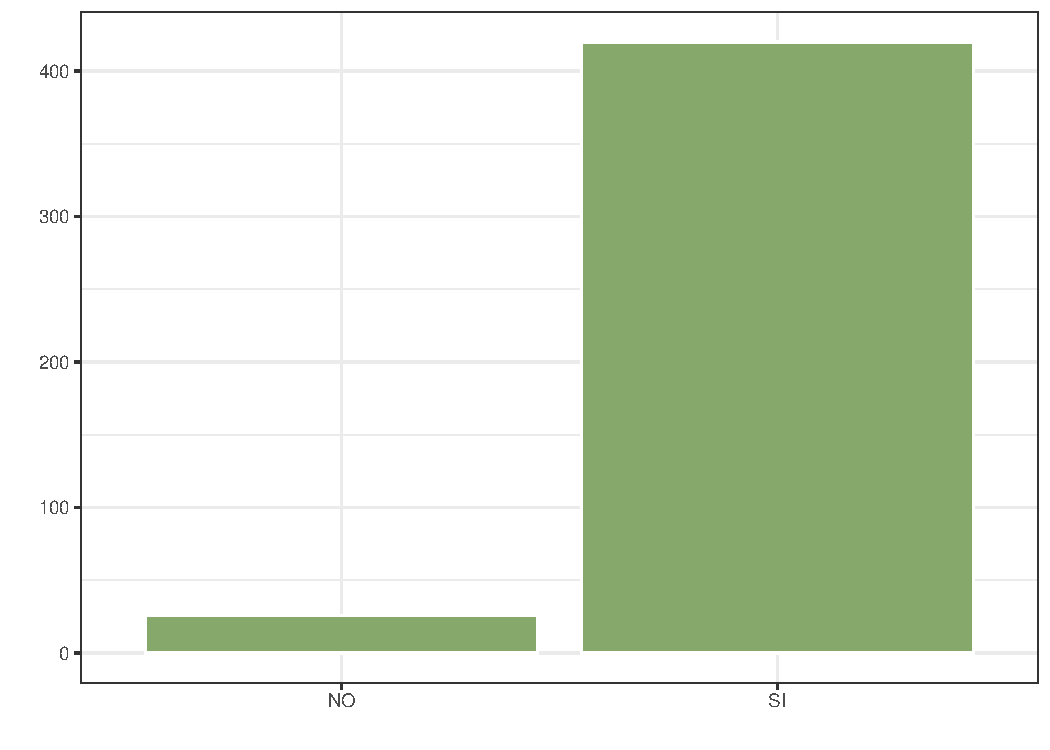
\includegraphics[width=\maxwidth]{figure/fig_doce-1} 
\end{knitrout}
  \caption*{Fuente: Trabajo de campo}
\end{figure}

\begin{figure}[H]
  \centering
  \caption{Sensibilizacion a los productores}
  \includegraphics[width=7cm, height=7cm]{H:/Gore Cusco/Geragri/programa/analisis datos/fotos/10.jpg}
  \caption*{Fuente: trabajo de campo}
\end{figure}






\begin{table}[H]
  \centering
  \caption{Energia electrica}

\begin{tabular}{lcl}
\toprule
\cellcolor[HTML]{87A96B}{\textcolor{black}{\textbf{area}}} & \cellcolor[HTML]{87A96B}{\textcolor{black}{\textbf{Conteo}}} & \cellcolor[HTML]{87A96B}{\textcolor{black}{\textbf{Porcentaje}}}\\
\midrule
0.01 HA & 2 & 0.45\\
0.06 HA & 1 & 0.23\\
0.07 HA & 1 & \vphantom{1} 0.23\\
0.1  HA & 1 & 0.23\\
0.1 HA & 4 & 0.90\\
\addlinespace
0.10 HA & 3 & 0.68\\
0.100 HA & 1 & 0.23\\
0.12 HA & 2 & 0.45\\
0.13 HA & 1 & 0.23\\
0.14 HA & 1 & 0.23\\
\addlinespace
0.15 HA & 7 & 1.58\\
0.2 H & 1 & 0.23\\
0.20 HA & 1 & 0.23\\
0.25 HA & 3 & 0.68\\
0.3 & 2 & 0.45\\
\addlinespace
0.3 HA & 4 & 0.90\\
0.30 H & 1 & 0.23\\
0.30 HA & 1 & 0.23\\
0.35 HA & 2 & 0.45\\
0.5 H & 1 & 0.23\\
\addlinespace
0.5 HA & 6 & 1.35\\
0.5 TOPO & 11 & 2.48\\
0.5 TOPOS & 1 & 0.23\\
0.6 H & 4 & 0.90\\
0.6 HA & 1 & 0.23\\
\addlinespace
1 & 3 & 0.68\\
1  TOPO & 1 & 0.23\\
1 1/2 HA & 1 & 0.23\\
1 1/2 TOPO & 6 & 1.35\\
1 H & 7 & 1.58\\
\addlinespace
1 HA & 13 & 2.93\\
1 HA Y 1 TOPO & 1 & 0.23\\
1 TOPO & 46 & 10.36\\
1 TPO & 1 & 0.23\\
1 topo & 1 & 0.23\\
\addlinespace
1.2 TOPO & 1 & 0.23\\
1.30 H & 1 & 0.23\\
1.5 & 1 & 0.23\\
1.5 H & 3 & 0.68\\
1.5 HA & 3 & 0.68\\
\addlinespace
1.5 TOPO & 2 & 0.45\\
1.5 TOPOS & 1 & 0.23\\
1/2  TOPO & 1 & 0.23\\
1/2 H & 1 & 0.23\\
1/2 HA & 18 & 4.05\\
\addlinespace
1/2 TOPO & 79 & 17.79\\
1/2 TOPOS & 1 & 0.23\\
1/4 & 1 & 0.23\\
1/4  TOPO & 1 & 0.23\\
1/4 HA & 1 & 0.23\\
\addlinespace
1/4 TOPO & 26 & 5.86\\
1/4 TOTAL & 1 & 0.23\\
1/4 h & 1 & 0.23\\
10 HA & 2 & 0.45\\
100 M & 5 & 1.13\\
\addlinespace
100 MTS2 & 1 & 0.23\\
1000 M & 3 & 0.68\\
1000 M2 & 1 & 0.23\\
1000 MTS & 1 & 0.23\\
12 HA & 2 & 0.45\\
\addlinespace
1200 MT & 1 & 0.23\\
12800 MT & 1 & 0.23\\
1400 MTS 2 & 1 & 0.23\\
15 HA & 2 & 0.45\\
1500 MT & 1 & 0.23\\
\addlinespace
1500 MTS & 1 & 0.23\\
1500 MTS 2 & 1 & 0.23\\
1OO M & 1 & 0.23\\
2 & 3 & 0.68\\
2 1/2 TOPO & 2 & 0.45\\
\addlinespace
2 HA & 14 & 3.15\\
2 TOPO & 3 & 0.68\\
2 TOPOS & 12 & 2.70\\
2.5 & 1 & 0.23\\
2.5 H & 1 & 0.23\\
\addlinespace
2.5 TOPOS & 1 & 0.23\\
20 HA & 2 & 0.45\\
200  M & 1 & 0.23\\
200 M & 1 & 0.23\\
200 MTS2 & 1 & 0.23\\
\addlinespace
2000 M & 1 & 0.23\\
2000 M2 & 1 & 0.23\\
2000 MTS 2 & 1 & 0.23\\
2000 MTS2 & 1 & 0.23\\
25 HA & 1 & 0.23\\
\addlinespace
2500 MT & 4 & 0.90\\
3 H & 1 & 0.23\\
3 HA & 4 & 0.90\\
3 TOPO & 2 & 0.45\\
3 TOPOS & 7 & 1.58\\
\addlinespace
3 TOPOS & 1 & 0.23\\
3/4 TOPO & 2 & 0.45\\
300 M & 2 & 0.45\\
300 MTS & 3 & 0.68\\
3000 MTS2 & 1 & 0.23\\
\addlinespace
3400 MT & 1 & 0.23\\
3700 M2 & 1 & 0.23\\
4  TOPOS & 1 & 0.23\\
4 HA & 6 & 1.35\\
4 TOPOS & 5 & 1.13\\
\addlinespace
400 MTS 2 & 1 & 0.23\\
400 MTS2 & 1 & 0.23\\
4000 MT & 1 & 0.23\\
4500 MT & 1 & 0.23\\
4543 MTS 2 & 1 & 0.23\\
\addlinespace
5 HA & 6 & 1.35\\
5 TOPO & 1 & 0.23\\
5 TOPOS & 4 & 0.90\\
5.5 & 1 & 0.23\\
5/8 TOPO & 1 & 0.23\\
\addlinespace
500 M & 1 & 0.23\\
500 M2 & 1 & 0.23\\
500 MT & 1 & 0.23\\
500 MTS & 1 & 0.23\\
5200 MTS2 & 1 & 0.23\\
\addlinespace
550MT & 1 & 0.23\\
6 HA & 2 & 0.45\\
6 TOPOS & 2 & 0.45\\
60 MTS2 & 1 & 0.23\\
600 MTS & 2 & 0.45\\
\addlinespace
6HA & 1 & 0.23\\
7 HA & 1 & 0.23\\
7 HA & 1 & 0.23\\
7000 MT & 1 & 0.23\\
71/2 HA & 1 & 0.23\\
\addlinespace
8 HA & 1 & 0.23\\
80 M & 1 & 0.23\\
800 M2 & 1 & 0.23\\
800 MTS 2 & 1 & 0.23\\
8000 M2 & 1 & 0.23\\
\addlinespace
8000 MT & 1 & 0.23\\
8000 MTS2 & 1 & 0.23\\
9 HA & 1 & 0.23\\
900 MTS2 & 1 & 0.23\\
PEQUEÑO & 1 & 0.23\\
\bottomrule
\end{tabular}

  \caption*{Fuente: Trabajo de campo}
\end{table}

\begin{figure}[H]
  \centering
  \caption{Energia electrica}
\begin{knitrout}
\definecolor{shadecolor}{rgb}{0.969, 0.969, 0.969}\color{fgcolor}
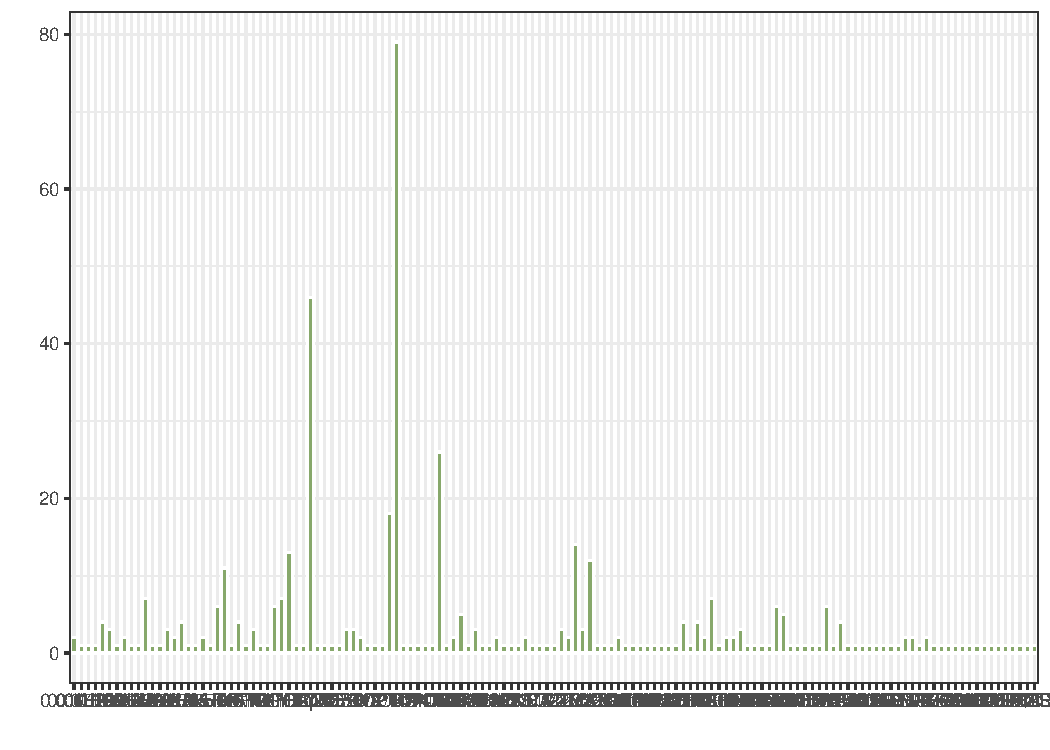
\includegraphics[width=\maxwidth]{figure/fig_trece-1} 
\end{knitrout}
  \caption*{Fuente: Trabajo de campo}
\end{figure}

\begin{figure}[H]
  \centering
  \caption{Sensibilizacion a los productores}
  \includegraphics[width=7cm, height=7cm]{H:/Gore Cusco/Geragri/programa/analisis datos/fotos/10.jpg}
  \caption*{Fuente: trabajo de campo}
\end{figure}
\end{document}
